\documentclass[11pt]{standalone}
\usepackage{amssymb}
\usepackage{amsmath}
\usepackage[no-math]{fontspec}
\usepackage{unicode-math}
\usepackage{libertinus}
\usepackage{pgf,xcolor}
\usepackage{tikz}
\usetikzlibrary{arrows.meta, backgrounds}
\usepackage{pgfplots}
\pgfplotsset{compat=newest}

\definecolor{my_darkgray}{HTML}{484949}
\definecolor{my_lightgray}{HTML}{F3F4F4}
\definecolor{my_darkblue}{HTML}{005A94}
\definecolor{my_lightblue}{HTML}{CCDEE9}
\definecolor{my_yellow}{HTML}{FFEC7F}
\definecolor{my_red}{HTML}{E60000}
\definecolor{my_orange}{HTML}{E87846}

\begin{document}
% ---------------------------------------------------------------
%  Entscheidungsweg fuer nichtlineare DGL 1. Ordnung: links die
%  Fragen in der Reihenfolge, in der wir sie stellen, rechts das
%  passende Verfahren. Unten der Fall ohne passende Bauart.
%  Koordinaten explizit gesetzt (keine positioning-Bibliothek,
%  damit die Praeambel unveraendert bleibt).
% ---------------------------------------------------------------
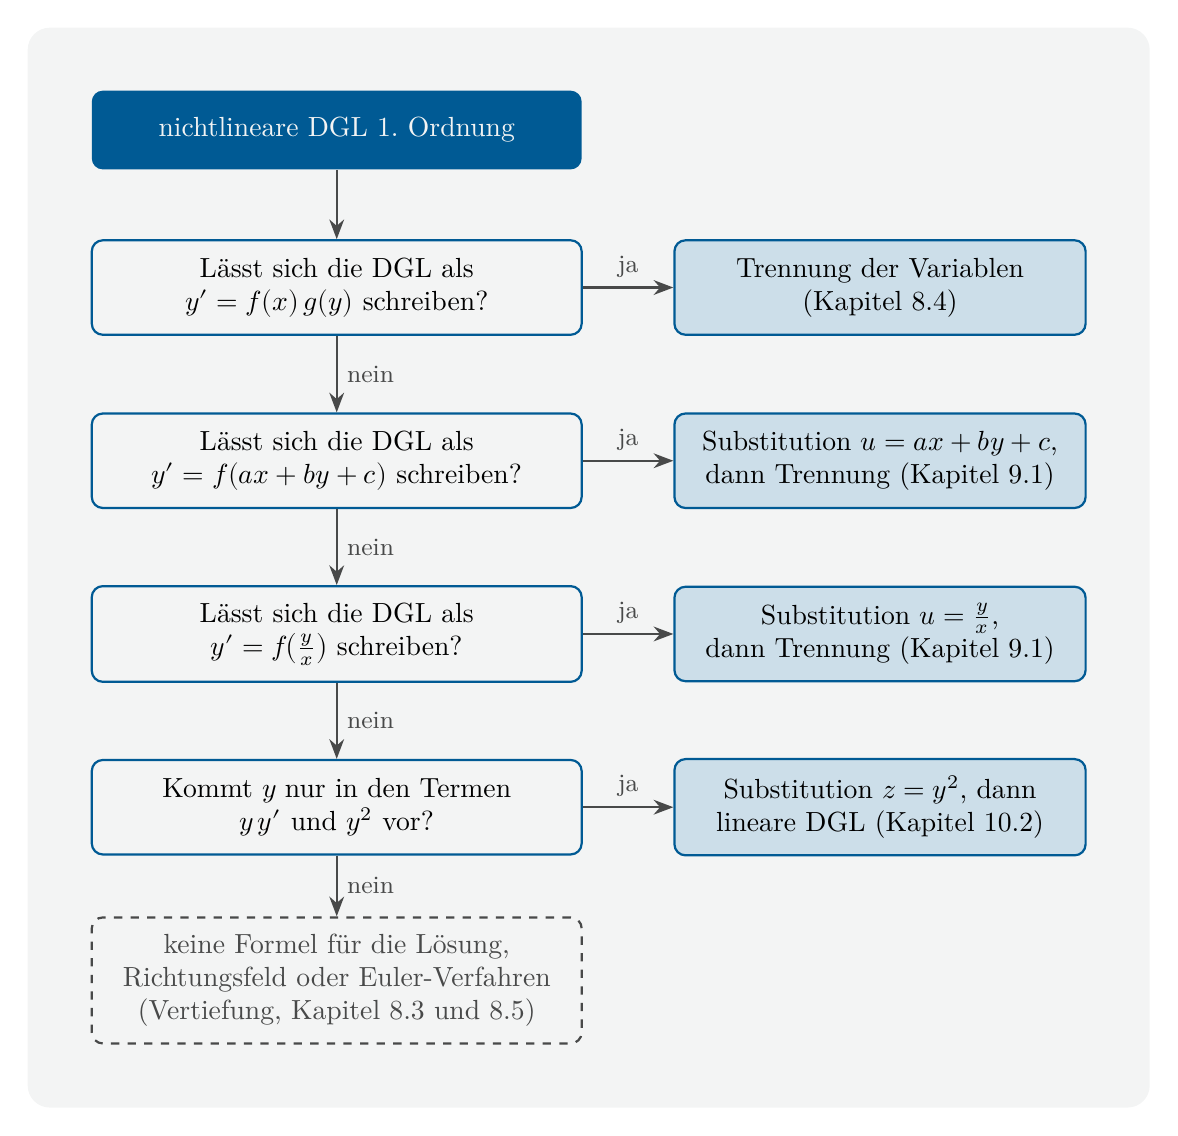
\begin{tikzpicture}[
    show background rectangle,
    background rectangle/.style={fill=my_lightgray, rounded corners=8pt},
    inner frame sep=0.8cm,
    start/.style={fill=my_darkblue, text=my_lightgray, rounded corners=4pt,
        text width=5.8cm, align=flush center, inner sep=6pt, minimum height=1cm},
    frage/.style={draw=my_darkblue, thick, rounded corners=4pt,
        text width=5.8cm, align=flush center, inner sep=6pt, minimum height=1.2cm},
    verfahren/.style={draw=my_darkblue, thick, fill=my_lightblue,
        rounded corners=4pt, text width=4.8cm, align=flush center, inner sep=6pt,
        minimum height=1.2cm},
    ende/.style={draw=my_darkgray, thick, dashed, rounded corners=4pt,
        text=my_darkgray, text width=5.8cm, align=flush center, inner sep=6pt,
        minimum height=1.2cm},
    pfeil/.style={-{Stealth[length=2.5mm]}, thick, my_darkgray},
    marke/.style={font=\small, text=my_darkgray},
]
\node[start] (s) at (0, 0) {nichtlineare DGL 1.~Ordnung};

\node[frage] (q1) at (0, -2)
    {Lässt sich die DGL als\\ $y' = f(x)\,g(y)$ schreiben?};
\node[verfahren] (m1) at (6.9, -2)
    {Trennung der Variablen\\ (Kapitel 8.4)};

\node[frage] (q2) at (0, -4.2)
    {Lässt sich die DGL als\\ $y' = f(ax + by + c)$ schreiben?};
\node[verfahren] (m2) at (6.9, -4.2)
    {Substitution $u = ax + by + c$,\\ dann Trennung (Kapitel 9.1)};

\node[frage] (q3) at (0, -6.4)
    {Lässt sich die DGL als\\ $y' = f\big(\frac{y}{x}\big)$ schreiben?};
\node[verfahren] (m3) at (6.9, -6.4)
    {Substitution $u = \frac{y}{x}$,\\ dann Trennung (Kapitel 9.1)};

\node[frage] (q4) at (0, -8.6)
    {Kommt $y$ nur in den Termen\\ $y\,y'$ und $y^2$ vor?};
\node[verfahren] (m4) at (6.9, -8.6)
    {Substitution $z = y^2$, dann\\ lineare DGL (Kapitel 10.2)};

\node[ende] (e) at (0, -10.8)
    {keine Formel für die Lösung,\\ Richtungsfeld oder Euler-Verfahren\\
     (Vertiefung, Kapitel 8.3 und 8.5)};

\draw[pfeil] (s) -- (q1);
\foreach \i/\j in {1/2, 2/3, 3/4}{
    \draw[pfeil] (q\i) -- node[marke, right] {nein} (q\j);
}
\draw[pfeil] (q4) -- node[marke, right] {nein} (e);
\foreach \i in {1, 2, 3, 4}{
    \draw[pfeil] (q\i) -- node[marke, above] {ja} (m\i);
}
\end{tikzpicture}
\end{document}
